\section{Spécifications fonctionnelles du projet}

Dans notre rapport précédent, nous définission un cahier des charges qui s'articulait principalement autour de 3 grands axes qui étaient les suivants : 
\begin{itemize}\renewcommand{\labelitemi}{$\bullet$}
\item Présence d'interactions avec l'environnement
\item Applications aisément portable vers différents systèmes d'utilisation
\item Exploitation de différents périphériques d'entrée/sortie
\end{itemize}
Nous allons donc dans un premier temps présenter les solutions techniques que nous avons retenues pour la réalisation du projet, en détaillant de quelle façon elles répondent à ces 3 problématiques, pour ensuite présenter un diagramme de cas d'utilisation qui résumera le fonctionnement global de l'application. 

\subsection{Solutions techniques retenues}
La réalisation de notre projet s'appuiera donc principalement sur trois environnements de travail, Unity3D, Blender et MiddleVR. 

\subsubsection{Unity : le moteur de rendu 3D}
L'utilisation d'Unity était imposée, en vertu des nombreux avantages du logiciel. Unity est un moteur de rendu 3D 
\begin{wrapfigure}{l}{0mm}
	\centering
	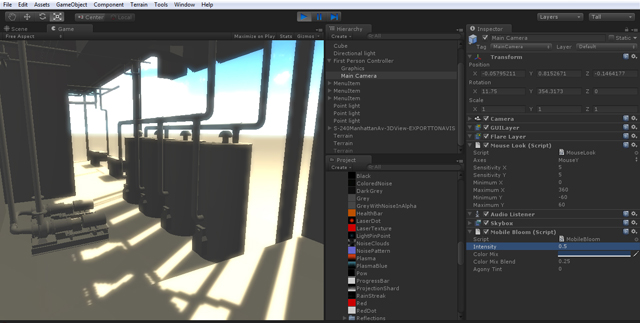
\includegraphics[scale=0.5]{2-Specifications/img-utilisateur/screen_unity.jpg}
\end{wrapfigure}
utilisé principalement pour la réalisation de jeux vidéos, et qui dispose d'une version gratuite. Très complet, il propose les différentes fonctionnalités dont nous avons besoin : il permet d'ouvrir le modèle 3D de l'appartement tremplin qui nous a été fourni par le centre de Kerpape, et de le modifier. \newline

Il permet aussi de réaliser les interactions entre utilisateur et environnement qui nous intéressent, que ce soit l'appui sur les différents interrupteurs gérant l'éclairage et l'ouverture/fermeture des volets, ou bien l'utilisation de la télécommande dont disposent les résidents de l'appartement qui centralise la plupart des actions qu'ils peuvent effectuer. 
Enfin dernier avantage de Unity, il propose différentes cibles de compilation. En effet, même si dans un premier temps nous allons développer une application qui fonctionnera sous Windows 7 ou 8 avec un ensemble clavier/souris, nous aimerions ne pas être limités à cet environnement par la suite. \newline

Néanmoins, un problème est survenu lors de l'utilisation de Unity : le modèle 3D de l'appartement qui nous avait été fourni avait été créé grâce à 3DSMax, et les deux logiciels sont réputés incompatibles entre eux, ce qui s'est avéré dans notre cas. Nous avons donc au final obtenu un modèle contenant les volumes, mais sans texture ni lumière, que nous avons dû ajouter nous-mêmes. 

\subsubsection{Blender : le logiciel de modélisation}
Blender est le logiciel de modélisation que nous allons utiliser pour les modifications du modèle qui nous a été fourni. Contrairement à Unity, il ne nous a pas été imposé, mais s'est dégagé comme étant le choix idéal du fait de la documentation imposante disponible sur le net et de sa gratuité.\newline

La majorité de l'appartement tremplin a déjà été modélisé pour nous, mais il reste néanmoins quelques détails à rajouter, comme l'interphone/téléphone (le domophone), ou encore le panneau d'interrupteurs à l'entrée de l'appartement. Nous nous en servirons de plus pour corriger les pertes rencontrées lors de l'import du modèle 3D sous Unity : rajouter la lumière et les textures à notre modèle. 

\subsubsection{MiddleVR : la gestion des périphériques d'interaction}

MiddleVR répond au troisième des objectifs que nous nous sommes fixés : exploiter différents périphériques d'entrée/sortie. En effet, pour ce faire, il fallait pouvoir s'abstraire desdits périphériques au cours du développement de l'application. L'idée est de développer toutes les fonctionnalités qui nous intéressent, l'utilisation des différents interrupteurs, etc, et d'ensuite disposer d'un moyen facile d'associer l'usage d'un périphérique donné à une fonctionnalité donnée.\newline

Or c'est précisément ce que nous permet MiddleVR. Prenant la forme d'un plugin Unity disponible gratuitement, il est capable de reconnaître les différents périphériques de réalité virtuelle à notre disposition, pour ensuite les associer à certaines actions.

\subsection{Scénarios d'utilisation}
Le cahier des charges qui nous a été fourni par le centre de Kerpape prévoit l'implémentation de différents scénarios d'utilisation centrés sur l'usage du domophone et que nous avons détaillés dans le premier rapport :
\begin{itemize}\renewcommand{\labelitemi}{$\bullet$}
\item Appel téléphonique normal
\item Appel \textit{via} l'interphone d'une personne venant fréquemment (un infirmier par exemple)
\item Appel \textit{via} l'interphone concernant une visite inattendue 
\end{itemize}
Ces scénarios mettent en avant l'usage particulier qui peut être fait du téléphone et de la télévision (cf. \textsc{figure~\ref{domophone}}), car ceux-ci servent d'interphone, respectivement pour le son et l'image. Il faut donc que le téléphone, dans notre application, puisse recevoir des appels des deux types différents, mais aussi que la TV puisse recevoir le flux vidéo de l'interphone (en pratique dans les appartements tremplins, l'habitant doit se placer sur le canal 80 pour afficher la caméra de l'interphone). 
\textbf{est-ce que ce passage est bien à sa place ici ???}
\begin{figure}[h!]
	\begin{center}
  		\caption{Cas d'utilisation du domophone}
  		\label{domophone}
  		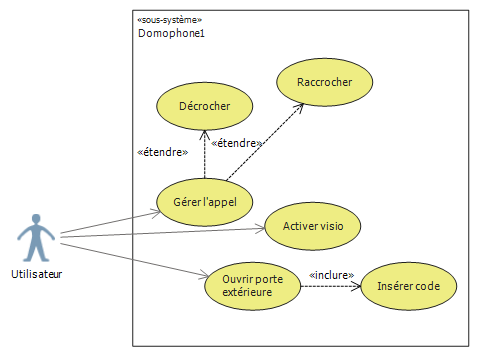
\includegraphics[scale=0.6]{2-Specifications/img-utilisateur/use_case_diag.PNG}
  	\end{center}
\end{figure}

\subsection{Déploiement}
Parmi nos 3 axes de développement, l'un était l'exploitation de différents périphériques d'entrée/sortie. Il y a, en pratique, 3 périphériques de sortie que nous prévoyons d'utiliser au cours du projet : un écran de PC classique, un casque de réalité virtuel type Occulus Rift, et la salle immersive Immersia de l'IRISA. 

\subsubsection{Ecran}
Il s'agit de la première version que nous allons développer. Cette version pourra reconnaître différents périphériques d'entrée, mais sera au départ prévue pour des interactions via le couple clavier/souris. Grâce à MiddleVR, cette option n'est pas plus ou moins facile à implémenter que les autres, mais elle représente un bon point de départ car elle ne nécessite pas d'équipement particulier, le centre de Kerpape disposant déjà de machines qui pourront faire tourner le programme. \newline

De  plus, bien que cette approche soit moins "naturelle" que l'usage de dispositifs de réalité virtuelle comme ceux associés à la salle Immersia, elle est au final aisée de prise en main car il s'agit de matériel auquel la plupart des gens sont déjà habitués. 

\subsubsection{Casque de RV}
La première approche présentée, bien qu'étant la plus pratique, n'implique pas suffisament la notion de réalité virtuelle qui est au coeur de notre projet. De plus, un dispositif comme un casque de réalité virtuelle permet une immersion plus totale de l'utilisateur. 
\begin{wrapfigure}{r}{0mm}
	\centering
	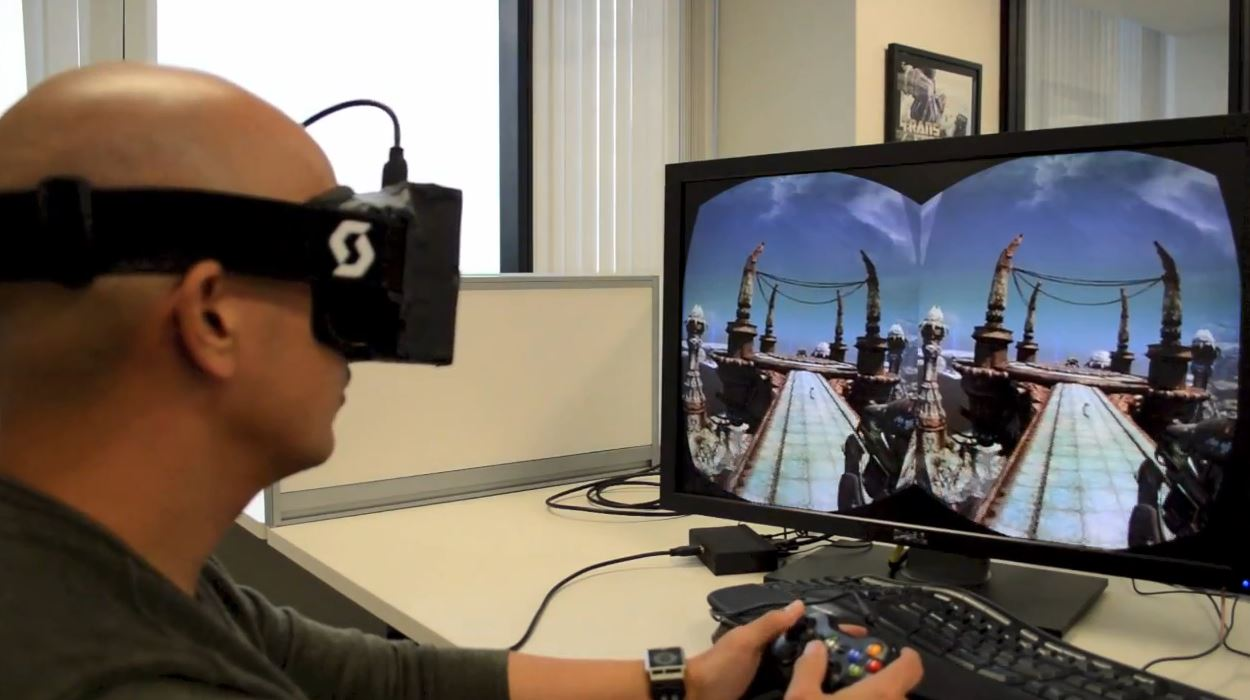
\includegraphics[scale=0.3]{2-Specifications/img-utilisateur/occulus.jpg}
\end{wrapfigure}
Qui plus est, elle se marie avantageusement avec l'usage de dispositifs comme des manettes pour Nintendo Wii ou des Razer Hydra qui sont eux-mêmes plus immersifs que le classique clavier/souris, car ils permettent de retranscrire les mouvements réels que l'utilisateur fera avec ses mains. \newline

Lors de notre visite au centre de Kerpape nous avons fait essayer une démonstration de l'Occulus Rift à Willy Allègre et Jean-Paul Departe, qui ont été plutôt convaincus de l'intérêt du dispositif. Néanmoins, il s'agit d'une technologie onéreuse et dont le centre ne dispose pas actuellement. 

\subsubsection{Salle immersive}
La salle immersive représente l'équipement de RV le plus complet dont nous puissions profiter et est donc une perspective de plate-forme très intéressante pour notre application. 
\begin{wrapfigure}{l}{0mm}
	\centering
	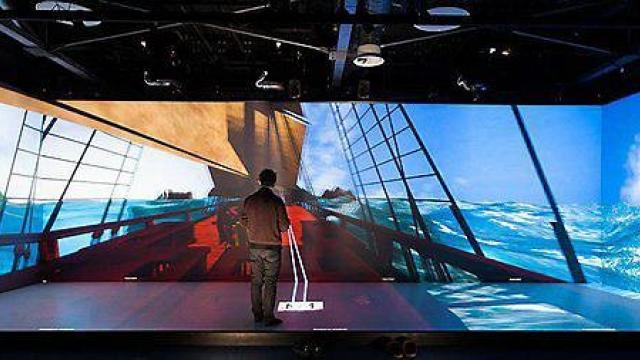
\includegraphics[scale=0.5]{2-Specifications/img-utilisateur/immersia.jpg}
\end{wrapfigure}
C'est l'option qui nous permettra les interactions les plus naturelles, car l'utilisateur se trouvera dans une projection à l'échelle 1:1 de l'appartement, équipé de lunettes 3D et de capteurs qui permettent de suivre la position des mains de l'utilisateur. \newline

Bien que Kerpape n'en dipose pas et n'ait pas la possibilité d'en utiliser une, l'implémentation du projet Avalon dans une salle immersive reste donc un objectif que nous souhaitons réaliser. 